\scanpage{35}
\mspage{I}
\margin{\figure{
\begin{tikzpicture}[x=1cm,y=1cm]
\fill (0,0)--(.06,.28)--(.03,.29)--(.10,.54)--(.05,.55)--(.10,.70)--(.04,.74)--(.09,.84)--(.18,.93)--(.21,1.02)--(.26,.94)--(.29,.78)--(.36,.72)--(.29,.70)--(.32,.60)--(.26,.62)--(.24,.56)--(.18,.56)--(.15,.35)--(.10,.29)--(.13,.24)--(.08,.03)--cycle;
\end{tikzpicture}}}
\begin{center}
Cohomologie des catégories de Banach
\figure{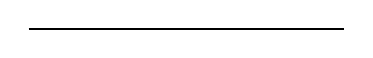
\begin{tikzpicture}\draw[line width=.7pt] (0,0)--(4,0);\end{tikzpicture}}
par Max Karoubi
\end{center}

Soit $\mathcal C$ une catégorie additive $^{(*)}$. Le \uline{groupe de Grothendieck} $K(\mathcal C)$ de la catégorie $\mathcal C$ est le quotient du groupe libre engendré par les classes d'isomorphie $\{G\}$ d'objets $G$ de $\mathcal C$ par le sous-groupe engendré par les relations $\{E+F\}-\{E\}-\{F\}=0$. Pour des applications topologiques du groupe de Grothendieck, voir par exemple $^{(1)}$. Dans cette note on se propose de définir de même, pour des catégories additives munies d'une certaine structure, des groupes $K^n(\mathcal C)$, $n\in Z$, avec $K^0(\mathcal C)\approx K(\mathcal C)$, jouissant de certaines propriétés ``cohomologiques'' en relation avec les théorèmes de périodicité de Bott.

I\qquad \uline{Définitions}

1.1\quad Une \uline{catégorie de Banach} (sous-entendu sur $k$ avec $k=\mathbb R$ ou $\mathbb C$) est la donnée d'une catégorie avec objet nul $\mathcal C$ et, quels que soient les objets $M$ et $N$ de $\mathcal C$, d'une structure de $k$-espace de Banach sur l'ensemble $\operatorname{Hom}_{\mathcal C}(M,N)$. Cette donnée est astreinte aux conditions suivantes :

a) Quels que soient les objets $M$, $N$ et $P$ de $\mathcal C$, l'application
\[
\operatorname{Hom}_{\mathcal C}(M,N)\times\operatorname{Hom}_{\mathcal C}(N,P)\longrightarrow\operatorname{Hom}_{\mathcal C}(M,P)
\]
définie par la composition des morphismes, est bilinéaire

\noindent\rule{\linewidth}{.4pt}

$(*)$ Toutes les catégories considérées ici sont des $\mathcal U$-catégories au sens de Grothendieck $^{(3)}$. Les objets d'une catégorie forment donc en particulier un ensemble.
\mspage{34}
